\documentclass{beamer}

\usepackage{amsmath}
\usepackage{amssymb}
\usepackage{framed}

\begin{document}
\section{Part 1}

\begin{frame}
%---------------------------------------------------- %
\begin{figure}
\vspace{1cm}
\centering

\includegraphics[width=0.99\linewidth]{./RlogoMAM}

%\label{fig:RlogoMAM}
\end{figure}
\LARGE
\[ \mbox{West of Ireland Data Science - Shiny Demonstration}  \]
\Large

\end{frame}
%---------------------------------------------------- %
\begin{frame}
\begin{figure}
\Large
\centering

\includegraphics[width=0.55\linewidth]{./Rstudio}
\[ \mbox{rstudio}  \]
%\label{fig:RlogoMAM}
\end{figure}

\end{frame}
\begin{frame}
%--------------------------------------------------%
\frametitle{RStudio}
\LARGE
\begin{itemize}
\item Makers of Shiny : RStudio\\ (JJ Allaire, Hadley Wickham etc etc) \bigskip
\item RStudio? IDE for \texttt{R}. \\ See \texttt{www.rstudio.org} for more.\bigskip
\item Shiny's  Lead Developers : Winston Chang and Joe Cheng.
\end{itemize}

\end{frame}
%---------------------------------------------------- %
\begin{frame}
\frametitle{Shiny - Slides Set 1}
\Large
\begin{itemize}
\item Overview of Demonstration
\item Resources (i.e. Shiny Tutorial Page)
\item Minimal Examples 
\item Widgets
\item A bit about JavaScript
\item Deploying Shiny
\end{itemize}
\end{frame}
%---------------------------------------------------- %

%---------------------------------------------%
%---------------------------------------------------- %
\begin{frame}
\Large
\frametitle{What is Shiny?}
\textbf{Easy web applications in R}\\
\textit{(Source: Shiny's Website)}
\begin{itemize}
\item \textbf{\textit{Shiny}} makes it super simple for \texttt{R} users like you to turn analyses into interactive web applications that anyone can use. \item Let your users choose input parameters using friendly controls like sliders, drop-downs, and text fields. \item Easily incorporate any number of outputs like plots, tables, and summaries.
\end{itemize}
\end{frame}
%---------------------------------------------------- %
%---------------------------------------------------- %
\begin{frame}
\Large
\frametitle{What is Shiny?}
\vspace{-1cm}
\textbf{Easy web applications in R (contd.)}\\
\textit{(Source: Shiny's Website)}
\begin{itemize}
\item No \textbf{HTML} or \textbf{JavaScript} knowledge is necessary. If you have some experience with \texttt{R}, you’re just minutes away from combining the statistical power of \texttt{R} with the simplicity of a web page.
\item \textit{(Remark: They do appear to be really handy - based on several examples  available on the internet!)}
\end{itemize}

\end{frame}
%---------------------------------------------------- %


%---------------------------------------------------- %
\begin{frame}
\Large
\frametitle{Shiny Resources}
\vspace{-1.5cm}
\textbf{Resources}
\begin{itemize}

\item Shiny Tutorial (\texttt{http://rstudio.github.io/shiny/tutorial}) \bigskip
\item Chris Beeley's New Book\\ (Sample Chapter Available) \bigskip
\item Stack-Overflow and GitHub 
\end{itemize}

\end{frame}
\begin{frame}
%---------------------------------------------------- %
\begin{figure}
\vspace{0.5cm}
\centering

\includegraphics[width=0.85\linewidth]{./snap2}

%\label{fig:RlogoMAM}
\end{figure}
\Large
\[ \mbox{Matthew Leonawicz (SNAP - Uni. Alaska Fairbanks)}  \]
\[\mbox{github.com/ua-snap/shiny-apps}‎\]
\[ \mbox{twitter.com/leonawicz} \]

\end{frame}

%---------------------------------------------------- %
\begin{frame}
\begin{figure}

\centering

\includegraphics[width=0.55\linewidth]{./github}
\[ \mbox{github - code sharing}  \]
%\label{fig:RlogoMAM}
\end{figure}
\Large


\end{frame}

\begin{frame}
\textbf{Showmeshiny.com}
	\begin{figure}
		
		\centering
		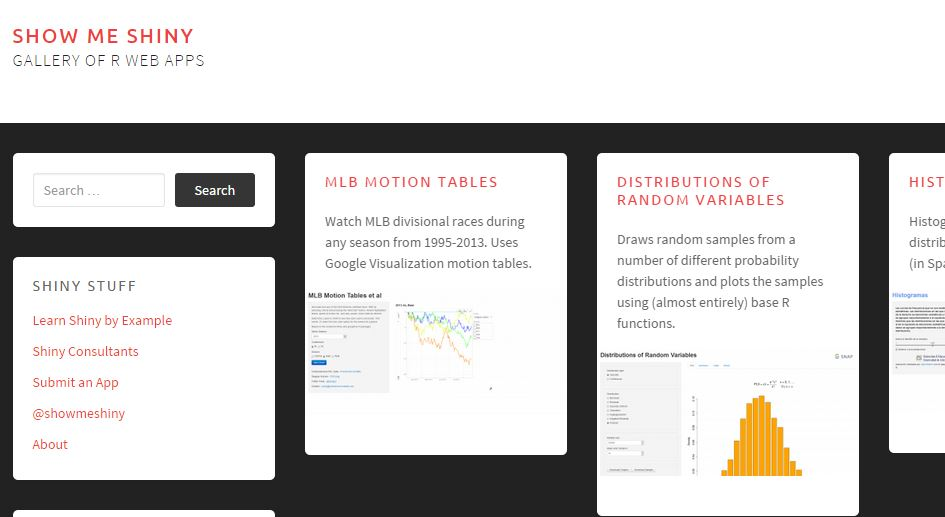
\includegraphics[width=0.95\linewidth]{./showmeshiny}
	
		%\label{fig:RlogoMAM}
	\end{figure}

	
	
\end{frame}


\section{Part 2}
%---------------------------------------------------- %
\begin{frame}
	\frametitle{Shiny - Part 2}
	\Large
	\textbf{Main Components of a Shiny Web App} 
	\begin{itemize}
		\item The shiny app is structurally a folder. The name of the app is the name of the folder.
		\item  Shiny programs are the easiest to build and
		understand using two scripts, which are kept within this folder. They must be
		named \texttt{server.R} and \texttt{ui.R}.
		\item 
		The input elements are defined in
		\texttt{ui.R} and processed by \texttt{server.R}, which then sends them back to \texttt{ui.R}
		\item Consideration: \textbf{\textit{Reactive Programming}}
	\end{itemize}
	
	
\end{frame}

%-----------------------------------------------%
\begin{frame}
	\frametitle{Shiny Basics}
	\Large
	\vspace{-0.5cm}
	\textbf{Basic structure of a Shiny program}
	\begin{itemize}
		\item  Selection of simple input widgets (checkboxes and radio buttons)
		\item  Selection of simple output types (rendering plots and returning text)
		\item  Selection of simple layout types (page with sidebar and tabbed output panel)
		\item  Handling reactivity in Shiny
	\end{itemize}
\end{frame}

%-----------------------------------------------%
\begin{frame}[fragile]
	\frametitle{Running a Shiny App}
	\Large
	To run a Shiny program on your local machine you just need to do the following:
	\begin{enumerate}
		\item  Make sure that \texttt{server.R} and \texttt{ui.R} are in the application subfolder (\texttt{appName}).
		\item Make the main folder \texttt{R}'s working directory (using the \texttt{setwd()} command, for
		example \texttt{setwd("~/shinyFiles")}).
		\begin{verbatim}
		>...\shinyFiles\appName
		\end{verbatim}
		\item Load the Shiny package (\texttt{library(shiny})). You
		should always do that in both \texttt{server.R} and \texttt{ui.R} files.
	\end{enumerate}
	
	
\end{frame}
%-----------------------------------------------%
\begin{frame}
	\frametitle{runApp}
	\Large
	\vspace{-1.5cm}
	\begin{itemize}
		\item Type \texttt{runApp("appName")} at the console.
		%\item runApp() with the name of a directory within works just as well, for example,runApp("~/shinyFiles/minimalExample").
		\item If you are in the application folder, just type \texttt{runApp()}
		\item \textbf{Important} - Just remember that it is a directory
		and not a file that you need to point to.
	\end{itemize}
\end{frame}
%-----------------------------------------------%
\begin{frame}
	\frametitle{ui.R}
	\Large
	\begin{itemize}
		\item The \texttt{ui.R} file is a description of the UI and is often the shortest and simplest part of
		a Shiny application. \item All of the UI elements are defined
		within this instruction.
		\item The standard shiny layout is a three panel layout, with a header panel, a sidepanel 
		controls on the left, and the main panel on the right - with the output.
		\item This layout is called \textbf{\emph{pageWithSidebar}}. There are other layouts too - such as basicPage and threePage.
	\end{itemize}
	
\end{frame}
%-----------------------------------------------%
\begin{frame}
	\Large
	%-----------------------------------------------%
	\frametitle{Inputs}
	The arguments are pretty typical among most of the widgets and are
	as follows:
	\begin{description}
		\item[ inputId]: This argument names the variable so it can be referred to in the
		\texttt{server.R} file
		\item[ label]: This argument gives a label to attach to the input so users know
		what it does
		\item[value]: This argument gives the initial value to the widget when it is
		set up. All the widgets should have sensible defaults for this argument.
	\end{description}
\end{frame}
%-----------------------------------------------%

%-----------------------------------------------%
\begin{frame}
	\frametitle{Main Panel}
	\Large
	\vspace{-1cm}
	\begin{itemize}
		\item The final function is \texttt{mainPanel()}, which sets up the output window. 
		\item  HTML helper functions - make a little title \texttt{h3("...")}. Knowledge of HTML is very useful!
		\item There are several of these functions designed to generate HTML to go straight on
		the page; \\e.g. type \texttt{?p} at the console for the complete list. 
	\end{itemize}
\end{frame}
%-----------------------------------------------%
%-----------------------------------------------%
\begin{frame}
	\Large
	\frametitle{Main Panel}
	\begin{itemize}
		\item The other element that goes in
		\texttt{mainPanel()} is an area for handling reactive text or plots generated within the\texttt{ server.R}
		file
		\item For example - a call to \texttt{textOutput()} with the name of the output as defined in
		\texttt{server.R}, in the upcoming "minimal case" examples.
		% "textDisplay".
	\end{itemize}
\end{frame}
%-----------------------------------------------%
\begin{frame}
	%-----------------------------------------------%
	\frametitle{server.R}
	\Large
	
	\begin{itemize}
		\item \texttt{shinyServer(...{...})} defines the bit of Shiny that's
		going to handle all the data. 
		\item On the whole, two types of things go in here. \item \textbf{Reactive
			objects} (for example, data) are defined, which are then passed around as needed (for
		example, to different output instructions), \item Outputs are defined, such as graphs.
	\end{itemize}
\end{frame}
%-----------------------------------------------%

%----------------------------------------------------- %
\section{Ractive Programming}
\begin{frame}[fragile]
	\Large
	\frametitle{Reactive Programming}
	
	Simple \texttt{R} example re: reactivity
	\begin{framed}
		\begin{verbatim}
		> A <- 5
		> B <- A + 3
		> A <-6         #Update A
		>
		> c(A,B,A+3)
		[1] 6 8 9
		>
		\end{verbatim}
	\end{framed}
	Compare this with Microsoft Excel Spreadsheets
\end{frame}
\end{document}
%---------------------------------------------------- %
%\section{Introduction}


\begin{figure}
\centering

\includegraphics[width=0.65\linewidth]{./github}

%\label{fig:RlogoMAM}
\end{figure}
\Large
\[ \mbox{GitHub}  \]

\end{frame}
